%%%
% Approach for Interactive Diagram-Specific
% Layout of Graph-based Software Diagrams
%%%

\chapter{Ansatz für das interaktive und diagrammspezifische Layout von graph-basierten Softwarediagrammen}
\label{chapter:interactive-approach}

In diesem Kapitel wird ein Ansatz für das interaktive und diagrammspezifische Layout von graph-basierten Diagrammen präsentiert. Zunächst werden im Abschnitt \ref{sec:criteria} die Kriterien für den Entwurf des Ansatzes aufgestellt. Eine kurze Übersicht der Funktionsweise wird im Abschnitt \ref{sec:functionality} gegeben. Im Abschnitt \ref{sec:interaction-mechanisms} werden die Mechanismen der Interaktion näher erläutert. Eine detaillierte Beschreibung der Layout-Patterns und deren Rolle in dem präsentierten Ansatz folgt im Abschnitt \ref{sec:layout-patterns}. Im Abschnitt \ref{sec:layout-calculation} wird erklärt, wie das Layout berechnet wird. Schließlich wird im Abschnitt \ref{sec:current-approaches-comparison} eine Abgrenzung zu bestehenden Ansätzen beschrieben.

%%%%%%%%%%%
% Critera %
%%%%%%%%%%%

\section{Kriterien}
\label{sec:criteria}

Im Folgenden werden Kriterien für den präsentierten Ansatz aufgestellt. Die Wahl der Kriterien stützt sich in erster Linie auf die Prinzipien für die agile Modellierung aus \cite{Ambler02Agile}. Weiterhin orientieren sich die Kriterien an den im Kapitel \ref{chapter:existing-approaches} vorgestellten Ansätzen, deren positiven Eigenschaften in die Auswahl einfließen.   Schließlich haben auch die ästhetischen Prinzipien (siehe Abschnitt \ref{sec:aesthetics-criteria}) sowie die Rahmenbedingungen dieser Arbeit (siehe Abschnitt \ref{sec:thesis-conditions}) einen Einfluss auf die gewählten Kriterien.

\begin{enumerate}[label={K.\arabic*}]
    \item \label{req:gui} \textbf{GUI} Wie bereits im Abschnitt \ref{sec:thesis-conditions} erwähnt, beschäftigt sich diese Arbeit ausschließlich mit Mechanismen für das Layout von Diagrammen, die in Tools für klassische grafische Benutzeroberflächen eingesetzt werden. Daher soll der Ansatz für klassische grafische Benutzeroberflächen ausgelegt sein und von üblichen GUI-basierten Bedientechniken wie z.B. \enquote{Drag and Drop} Gebrauch machen.
    \item \label{req:interactivity} \textbf{Interaktivität} Die Manipulation mit dem Diagramm soll interaktiv erfolgen. Der Nutzer soll in der Lage sein, mit dem Diagramm unmittelbar interagieren zu können und die Layout-Anpassungen sollen eine direkte Auswirkung auf das manipulierte Diagramm haben. Demzufolge soll die Eingabe mit der Ausgabe fest gekoppelt sein\footnote{Dies bezieht sich auf das GUI-Tool, das den Ansatz implementiert. Aus der Sicht der Mensch-Computer-Interaktion ist die Nutzung der Maus als Eingabegerät von der Ausgabe am Monitor stets entkoppelt.}.
    % TODO: Fußnote verbessern!
    
    \item \label{req:immediate-feedback} \textbf{Unmittelbares Feedback} \cite[S.69]{Wybrow08Using}
    \item \label{req:editing-support} \textbf{Förderung des Prozesses der Diagramm-Erstellung} Der Nutzer soll den Inhalt des Diagramms bearbeiten und inkrementell modifizieren können \cite{GladischSchumann14Semi-Automatic}. Dabei soll das Layout nach jeder Änderung des Inhalts angepasst werden. Weiterhin soll es möglich sein, das Layout des Diagramms bis zu einem bestimmten Grad nach den Präferenzen des Nutzers beeinflussen zu können.
    \item \label{req:mental-map} \textbf{Erhaltung des mentalen Modells} Die Layout-Änderungen im Diagramm sollen möglichst intuitiv erfolgen, insbesondere soll das mentale Modell erhalten werden (siehe Abschnitt \ref{subsec:mental-map}).
    \item \label{req:focus-on-the-content} \textbf{Förderung der Konzentration auf den Inhalt} Der Inhalt eines Diagramms soll eine wichtigere Rolle als seine Repräsentation haben \cite[S.38ff]{Ambler02Agile}. Diese Tatsache soll in dem Ansatz berücksichtigt werden, indem der Aufwand für das Erzeugen des Layouts verringert wird. Außerdem sollen die Aktionen zur Anpassung der visuellen Eigenschaften möglichst eingeschränkt sein.
    \item \label{req:aesthetics-criteria} \textbf{Berücksichtigung der ästhetischen Prinzipien} Die Layout-Berechnung soll unter Berücksichtigung der im Abschnitt \ref{sec:aesthetics-criteria} beschriebenen ästhetischen Prinzipien für graph-basierte Softwarediagramme erfolgen.
    \item \textbf{Berücksichtigung der Syntax und Semantik} Die Syntax- und Semantikregeln der einzelnen Diagrammtypen sollen berücksichtigt werden und die Möglichkeit der Verletzung der Regeln sollte verhindert werden.
       
%    \item \label{req:user-friendly} \textbf{Benutzerfreundlichkeit} Der Ansatz soll möglichst benutzerfreundlich sein. Insbesondere ist wichtig, dass die Einschränkungen bzgl. des Layouts nicht zur Frustration des Nutzers führen.
\end{enumerate}

%%%%%%%%%%%%%%%%%
% Functionality %
%%%%%%%%%%%%%%%%%

\section{Funktionsweise}
\label{sec:functionality}

Der präsentierte Ansatz operiert auf dem Modell der konkreten Syntax einer graph-basierten visuellen Sprache und berechnet die Layout-Eigenschaften für Knoten und Kanten eines Diagramms (siehe Abschnitt \ref{subsec:graph-based-diagrams}). Die Berechnung erfolgt \textbf{halbautomatisch}, denn der Nutzer kann den Layout-Prozess durch die Interaktion mit dem Diagramm beeinflussen. Dabei wird versucht, ein optimales Verhältnis zwischen der Möglichkeit der flexiblen Modifizierung der Layout-Eigenschaften durch den Nutzer und einer automatisierten Layout-Berechnung zu erreichen. Der Ansatz kombiniert die Vorteile des manuellen und automatischen Layouts und lässt sich daher in die Gruppe der Ansätze für das interaktive halbautomatische Layout einordnen (siehe Abschnitt \ref{sec:interactive-semi-automatic-layout}).

Die Interaktion des Nutzers mit dem Diagramm erfolgt durch die Ausführung von \textbf{Bearbeitungsaktionen}, die mit Hilfe von \textbf{Bedienungsmechanismen} im Diagram realisiert und veranschaulicht werden. Für jede Bearbeitungsaktion werden ein oder mehrere \textbf{Layout-Ereignisse} erzeugt, die Informationen über die manipulierten Objekte sowie über die Parameter der Interaktion wie z.B. Position des Mauszeigers kapseln. Die erzeugten Layout-Ereignisse werden durch eine \textbf{Layout-Engine} ausgewertet, die für den Typ des Diagramms speziell angepasst ist. Intern verwaltet sie Instanzen von \textbf{Layout-Patterns}, die die Struktur des Diagramms beschreiben. Anhand des aktuellen Inhalts und Layouts des Diagramms und der instanziierten Layout-Patterns wird eine Anpassung des Layouts berechnet, die auf das Diagramm angewendet wird, wobei der Layout-Übergang visualisiert wird.

%%%%%%%%%%%%%%%%%%%%%%%%%%
% Interaction Mechanisms %
%%%%%%%%%%%%%%%%%%%%%%%%%%

\section{Mechanismen der Interaktion}
\label{sec:interaction-mechanisms}

Das Kriterium \ref{req:editing-support} erfordert eine Möglichkeit der Bearbeitung des Diagramms. Der Nutzer soll in der Lage sein, neue Knoten und Kanten hinzuzufügen und bestehende Knoten und Kanten zu manipulieren bzw. zu löschen. Durch das Kriterium \ref{req:interactivity} wird gefördert, dass die Bearbeitung interaktiv erfolgt. Dies wird durch die Unterstützung von \textbf{Bearbeitungsaktionen} gewährleistet, die die Grundlage der Interaktion bilden. Die Bearbeitungsaktionen werden im Abschnitt \ref{subsec:edit-actions} im Detail beschrieben.

Weiterhin sollen die Möglichkeiten der Interaktion eingeschränkt werden, um das Ablenken durch die Layout-Anpassungen zu minimieren (Kriterium \ref{req:focus-on-the-content}). Dies wird durch die Einschränkung der freien Positionierung der Knoten und den Einsatz eines \textbf{neuen Bedienungsmechanismus} für die Verschiebungsoperation erreicht, dem sich der Abschnitt \ref{subsec:temporary-layer-mechanism} widmet.

Die Erhaltung des mentalen Modells (Kriterium \ref{req:mental-map}) wird durch eine \textbf{Animation der Layout-Übergänge} gefördert, das im Abschnitt \ref{subsec:animation-interaction} behandelt wird.

% TODO: Die Einführung nochmal nach dem Fertigstellen der Bearbeitungsaktionen überprüfen

\subsection{Bearbeitungsaktionen}
\label{subsec:edit-actions}

Die interaktiven Ansätze werden in Editoren eingesetzt, die in der Regel über einen \enquote{Canvas} verfügen. Der Canvas ist ein rechteckiger Bereich des Editor-Fensters, in dem das Diagramm dargestellt wird und in dem die Interaktion mit dem Diagramm stattfindet. Die Interaktion setzt sich aus Bearbeitungsaktionen zusammen, die durch den Nutzer ausgeführt werden. Um das Kriterium \ref{req:gui} zu erfüllen, sollen alle Bearbeitungsaktionen auf GUI-Techniken basieren.

In dieser Arbeit werden die grundlegenden Bearbeitungsaktionen präsentiert, die insbesondere für die Entwicklung des Prototyps (siehe Kapitel \ref{chapter:prototype}) eine wichtige Rolle spielen. Natürlich ist eine Erweiterung der unterstützten Bearbeitungsaktionen möglich.

Je nach der Art der Modifizierung lassen sich die Bearbeitungsaktionen in zwei Gruppen unterteilen. Zu einem sind das Aktionen, die den Inhalt des Diagramms modifizieren (z.B. Hinzufügen oder Löschen eines Knotens) und zu anderem sind das Aktionen, die das Layout des Diagramms modifizieren, ohne den Inhalt zu verändern (z.B. Verschiebung eines Knotens). Beide Gruppen und deren Vertreter werden in den Abschnitten \ref{subsubsec:edit-actions-content-modification} und \ref{subsubsec:edit-actions-layout-modification} vorgestellt.

\subsubsection{Bearbeitungsaktionen zur Modifizierung des Inhalts}
\label{subsubsec:edit-actions-content-modification}

%\paragraph{Hinzufügen einer Kante}

%Eine Kante in graph-basierten Diagrammen verbindet genau zwei Knoten, wobei es sich entweder um eine Verbindung zwischen zwei unterschiedlichen Knoten oder von einen Knoten mit sich selbst handelt. 

% verzögertes Feedback?

\subsubsection{Bearbeitungsaktionen zur Modifizierung des Layouts}
\label{subsubsec:edit-actions-layout-modification}

% freie Positionierung
% Verschiebungsaktion -> gewünschte Position
% unmittelbares Feedback?

\subsection{Mechanismus der temporären Schicht}
\label{subsec:temporary-layer-mechanism}

\subsection{Animation der Layout-Übergänge}
\label{subsec:animation-interaction}
% \ref{req:mental-map}

%%%%%%%%%%%%%%%%%%%
% Layout Patterns %
%%%%%%%%%%%%%%%%%%%

\section{Layout-Patterns}
\label{sec:layout-patterns}

\subsection{Implizite Layout-Patterns}
\label{subsec:implicit-layout-patterns}

\subsubsection{Größe der Knoten}
\subsubsection{Zentrierung des Inhalts}
\subsubsection{Gleiche Abstände}
\subsubsection{Verhinderung der Knoten-Überlappung}

\subsection{Explizite Layout-Patterns}
\label{subsec:explicit-layout-patterns}

\subsubsection{Ausrichtungspattern}
\subsubsection{T-Shape-Pattern}

%%%%%%%%%%%%%%%%%%%%%%
% Layout Calculation %
%%%%%%%%%%%%%%%%%%%%%%

\section{Berechnung des Layouts}
\label{sec:layout-calculation}

%%%%%%%%%%%%%%%%%%%%%%%%%%%%%%%%%
% Current Approaches Comparison %
%%%%%%%%%%%%%%%%%%%%%%%%%%%%%%%%%

\section{Abgrenzung zu bestehenden Ansätzen}
\label{sec:current-approaches-comparison}

%%%%%%%%%
\endinput 
%%%%%%%%%

\subsection{Bearbeitungsaktionen}
\label{subsec:edit-actions}

Alle interaktiven Ansätze für das Layout von Diagrammen aus dem Kapitel \ref{chapter:existing-approaches} bis auf das \enquote{Smart Layout} in MindNode (siehe Abschnitt \ref{subsubsec:smart-layout-in-mindnode}) unterstützen die \textbf{freie Positionierung} der Objekte im Diagramm. Diese Art der Bedienung wird im manuellen Layout zusätzlich um temporäre Hilfefunktionen (siehe Abschnitt \ref{sec:manual-layout}) und in Struktur-basierten benutzergesteuerten Ansätzen um Möglichkeit der Erzeugung von Strukturregeln (siehe Abschnitt \ref{subsec:structure-based-user-controlled-approaches}) erweitert. Durch diese Erweiterungen wird die freie Positionierung eingeschränkt, dass in der Regel zu einem besseren Layout des Diagramms führt. Dahingegen ist die freie Positionierung in \enquote{Smart Layout} in MindNode und dem in dieser Arbeit präsentierten Ansatz \textbf{nicht gestattet}. Somit bewirkt die Verschiebung eines Objekts im Diagramm keine direkte Anpassung seiner Position, sondern wird als eine Äußerung der gewünschten Position interpretiert.

\subsection{Mechanismus der temporären Schicht}

Die interaktiven Ansätze werden in Editoren eingesetzt, die in der Regel über einen \enquote{Canvas} verfügen. Der Canvas ist ein rechteckiger Bereich des Editor-Fensters, in dem das Diagramm dargestellt wird und in dem die Interaktion mit dem Diagramm stattfindet. Obwohl in den meisten Editoren die Reihenfolge der Objekte im Canvas festgelegt werden kann und der Canvas somit mehrschichtig erscheint, handelt es sich aus der Sicht der Interaktion lediglich um \textbf{eine Schicht}, in der die Bearbeitungsaktionen ausgeführt werden. Dies ist der Fall für alle im Kapitel \ref{chapter:existing-approaches} vorgestellten interaktiven Ansätze und deren Implementierungen\footnote{Eine Ausnahme bildet das Hinzufügen von Objekten durch Verschiebung aus einer Palette in Programmen wie z.B. Keynote und Visual Paradigm.}.

Für die Umsetzung der Bearbeitungsaktionen unter Berücksichtigung der Einschränkung der freien Positionierung der Objekte war der Entwurf eines \textbf{neuen Bedienungsmechanismus} erforderlich. Dieser Mechanismus bildet die Grundlage des gesamten Ansatzes und wird im Folgenden anhand eines Beispiel der Verschiebungsaktion im Detail erklärt.

Die Verschiebungsaktion bewirkt die Verschiebung eines Objekts im Diagramm. Sie basiert auf der Technik \textbf{\enquote{Drag and Drop}} und ist in drei Phasen aufgeteilt.

Bevor die Verschiebung beginnen kann, müssen sich im Canvas einige Objekte befinden, so wie es der Fall in Abbildung \ref{fig:movement-action-example-a} ist.

\begin{figure}[hbt]
    \newcommand{\subfigurewidth}{0.28\textwidth}
    \newcommand{\graphicsscale}{1.2}
    \centering
    \begin{subfigure}{\subfigurewidth}
        \centering
        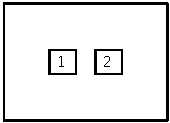
\includegraphics[scale=\graphicsscale]{resources/movement-action-example-a}
        \caption{}
        \label{fig:movement-action-example-a}
    \end{subfigure}
    \begin{subfigure}{\subfigurewidth}
        \centering
        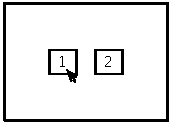
\includegraphics[scale=\graphicsscale]{resources/movement-action-example-b}
        \caption{}
        \label{fig:movement-action-example-b}
    \end{subfigure}
    \begin{subfigure}{\subfigurewidth}
        \centering
        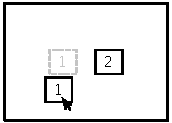
\includegraphics[scale=\graphicsscale]{resources/movement-action-example-c}
        \caption{}
        \label{fig:movement-action-example-c}
    \end{subfigure}
    \begin{subfigure}{\subfigurewidth}
        \centering
        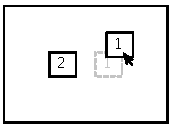
\includegraphics[scale=\graphicsscale]{resources/movement-action-example-d}
        \caption{}
        \label{fig:movement-action-example-d}
    \end{subfigure}
    \begin{subfigure}{\subfigurewidth}
        \centering
        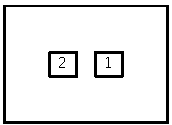
\includegraphics[scale=\graphicsscale]{resources/movement-action-example-e}
        \caption{}
        \label{fig:movement-action-example-e}
    \end{subfigure}
    \caption{Beispiel einer Verschiebungsaktion}
    \label{fig:movement-action-example}
\end{figure}

In der ersten Phase wird ein Objekt im Canvas angeklickt, das in Abbildung \ref{fig:movement-action-example-b} durch einen Mauszeiger gekennzeichnet ist. Dabei wird das angeklickte Objekt in eine neu eingefügte \textbf{temporäre Schicht} ausgelagert, die vor dem Canvas positioniert ist. Eine Visualisierung der Schichten ist in Abbildung \ref{fig:temporary-layer-visualization} nachzuschauen. Im Canvas wird die ursprüngliche Darstellung des verschobenen Objekts durch ein \textbf{temporäres Platzhalter-Objekt} ausgetauscht, das dem Nutzer die Zielposition des verschobenen Objekts andeutet. Das Platzhalter-Objekt ist in Abbildung \ref{fig:movement-action-example-c} durch ein Rechteck repräsentiert, das mit einer grauen gestrichelten Linie umrandet ist.

% TODO: Mauszeiger hinzufügen
\begin{figure}[hbt]
    \newcommand{\subfigurewidth}{0.35\textwidth}
    \newcommand{\graphicsscale}{1.2}
    \centering
    \begin{subfigure}{\subfigurewidth}
        \centering
        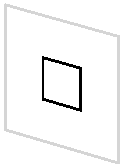
\includegraphics[scale=\graphicsscale]{resources/temporary-layer-visualization-a}
        \caption{}
    \end{subfigure}
    \begin{subfigure}{\subfigurewidth}
        \centering
        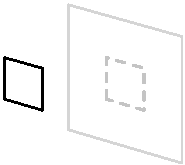
\includegraphics[scale=\graphicsscale]{resources/temporary-layer-visualization-b}
        \caption{}
    \end{subfigure}
    \caption{Darstellung der temporären zweiten Schicht}
    \label{fig:temporary-layer-visualization}
\end{figure}

In der zweiten Phase findet eine Bewegung des Mauszeigers statt. Da die temporäre Schicht an den Mauszeiger gebunden ist, wird die ausgelagerte Darstellung des Objekts frei mit dem Mauszeiger bewegt, währenddessen das Platzhalter-Objekt im Canvas seine Position zunächst nicht ändert. Dies ist in Abbildung \ref{fig:movement-action-example-c} illustriert.

Durch die Positionierung des Mauszeigers wird die gewünschte Position des verschobenen Objekts geäußert, die nach jeder Bewegung intern ausgewertet wird. Sobald sich der Mauszeiger in einem bestimmten Bereich befindet, für den das Layout des Diagramms geändert werden soll, wird das Layout im unterliegenden Canvas animiert angepasst. Dabei wird die Änderung der Layout-Eigenschaften des verschobenen Objekts auf das Platzhalter-Objekt angewendet, so wie es in Abbildung \ref{fig:movement-action-example-d} dargestellt ist. Durch die Anpassung des Layouts während der Interaktion wird ein unmittelbares Feedback erreicht (Kriterium \ref{req:immediate-feedback}) und die Animation sorgt für die Erhaltung des mentalen Modells (Kriterium \ref{req:mental-map}). Wie die Auswahl des Layouts intern konkret funktioniert wird im Abschnitt X beschrieben.

Nach dem Loslassen der Maustaste springt das verschobene Objekt auf die Zielposition hin, die durch die Position des Platzhalter-Objekts bestimmt ist. Anschließend werden das Platzhalter-Objekt sowie die temporäre Schicht entfernt und die Verschiebungsaktion wird beendet. Die Abbildung \ref{fig:movement-action-example-e} zeigt den Endzustand.

% Im Unterschied wird das Layout in MindNode erst nach dem Loslassen der Maustaste angepasst und stellt damit ein verzögertes Feedback dar.

% TODO: Zusammenfassung schreiben
% Der Mechanismus ist für klassische grafische Benutzeroberflächen ausgelegt und erfüllt damit das Kriterium \ref{req:gui}.


\subsection{Layout-Engine}

Nach dem Ausführen einer Bearbeitungsaktion (siehe Abschnitt \ref{subsec:edit-actions}) bzw. ihres Teils durch den Nutzer wird ein Layout-Ereignis erzeugt, das neben der Information über die manipulierten Objekte auch Parameter der Interaktion wie z.B. die Position des Mauszeigers besitzt.


% Layout-Übergänge

% Auswertung der Verschiebungsaktion
% ursprünglicher Ansatz





% Einschränkung der Aktionen, die der Nutzer ausführen kann

% Abnehmen der Layout-Arbeit durch Einschränkung der Flexibilität

% Herausforderung bei der Kombination von mehreren Kriterien (z.B. interaktive Bedienung aber gleichzeitig eine Einschränkung der Möglichkeiten)




%%%%%%%%%

% Meta-Modell
% Klassendiagramme meistens weniger als 10 Klassen (Rat von Scott Ambler?)
% Durch die Spezialisierung auf konkrete Diagramm-Typen und den Einsatz von verschiedenen Vereinfachungsmaßnahmen wie etwa Einschränkung der unterstützten Notation \cite[S.56ff]{Ambler02Agile} lassen sich Algorithmen für das Layout von Softwarediagrammen entwerfen, die zwar nicht so flexibel wie z.B. \cite{Maier12A-Pattern-based} oder \cite{Eichelberger05Aesthetics} sind, aber dafür...



% Layout-Engine
% =============
% Eingabe für den Algorithmus: Layout-Ereignis, Inhalt des Diagramms, instanziierte Patterns, der Layout-Zustand (mögliche Layout-Übergänge vom aktuellen Zustand abhängig, nicht alle erreichbar)
% berechnete Layouts = Positionen für Knoten, Routen für Kanten (nicht implementiert), Animationen/Übergangsparameter für die Transitionen (nicht implementiert)
% initialer Zustand

% Erreichbare Layouts werden berechnet und mit Hilfe der Layout-Ereignisse wird geprüft, ob ein Layout-Übergang stattfinden soll (z.B. nur die benachbarten Bereiche im horizontalen Layout-Algorithmus)
% nach einem Layout-Übergang wird die Berechnung wiederholt

% Layout-Engine soll für spezielle Diagrammtypen unterschiedliches Verhalten aufweisen
% Jeder Diagrammtyp (z.B. Klassendiagramm, Zustandsdiagramm, Flowchart usw.) hat aufgrund der Semantik- und Strukturregeln spezielle Anforderungen an das ästhetische Layout
% automatische Instanziierung von Patterns nach Layout-Ereignissen
% Neu-Berechnung nach jedem Layout-Übergang -> Performance?
% Stabilität -> Ausführen eines Layout-Übergangs nach einer deutlichen Aktion des Nutzers
% Erreichbarkeit des Ausgangslayouts

% In Rahmen der Konzeption und Entwicklung wurde zunächst ein Algorithmus entworfen, der für die Manipulation eines Knotens alle möglichen Layouts und die entsprechenden Diagramm-Bereiche für das gesamte Diagramm explizit berechnet hat. Durch eine Bewegung des Mauszeigers in einen anderen Bereich wurde jeweils ein Layout-Übergang ausgelöst. Die Berechnung wurde jedoch nicht nach jedem Layout-Übergang wiederholt und die Abbildung war oft nach dem ersten Layout-Übergang ungültig. Später wurde festgelegt, dass dieser Algorithmus nicht hinreichend ist.

\section{Layout-Patterns}
\label{sec:layout-patterns}

% Abgrenzung des Begriffs zu dem von [Maier]
% implizite vs. explizite Layout-Patterns (siehe Mappe)
% Patterns-Variierung (z.B. Reihenfolge der Knoten kann von Nutzer festgelegt werden, das endgültige Layout wird durch die Geometrie bestimmt)
% instanziiert in der Layout-Engine, referenzieren den Diagramm-Inhalt
% Wiederverwendung möglich (mehrere Instanzen in der Layout-Engine bzw. Komposition von Patterns wie T-Shape-Pattern)
% Nur während Drag&Drop sichtbar -> Möglichkeit der Interaktivität der Patterns
% interne Berechnung des relativen Layouts für enthaltene Diagramm-Objekte (Knoten)

% konkrete Pattens:
% - detaillierte Beschreibung der expliziten Layout-Patterns mit Bezug auf Arbeiten
% - Erläutern der geometrischen Parametern mit Bildern
% - Bild mit Instanzen von Patterns in einem Beispiel-Diagramm (kann ein Screenshot sein)
% - IDLPattern, IDLAlignmentPattern, IDLTShapePattern -> Klassendiagramm

% Offene Fragen
% =============
% Visualisierung
% Instanziierung durch den Nutzer wie in [Maier] ist denkbar

\subsection{Implizite Layout-Patterns}

\subsubsection{Größe der Knoten}
\subsubsection{Zentrierung des Inhalts}
\subsubsection{Gleiche Abstände}
\subsubsection{Verhinderung der Knoten-Überlappung}

\subsection{Explizite Layout-Patterns}

% TODO: Verweis auf die implementierten Patterns im Prototypen (Kapitel 5) hinzufügen
% Variationen der expliziten Layout-Patterns

\subsubsection{Ausrichtung}

% siehe manuelles Layout bzw. Pattern-basierter Ansatz (Kapitel 3)
% gleichmäßige Verteilung (Abstände gleich groß)
% Variationen: Reihenfolge der Knoten

\subsubsection{T-Shape}

% Variationen: Reihenfolge der Knoten im Ausrichtungs-Pattern
% interne Wiederverwendung eines Ausrichtung-Patterns

\section{Abgrenzung zu bestehenden Ansätzen}

% Was ist neu an dem Ansatz?
% Vergleich zu bestehenden Ansätzen im Kapitel 3
% Worin unterscheidet sich mein Ansatz zu dem von Sonja Maier?
% - \enquote{Drag and Drop} mit Visualisierung der Aktion
% - Kein Freihand-Editieren, sondern implizite Bereiche und Layout-Übergänge
% - Patterns unterstützen Variierung
% - Starke Vereinfachung der Möglichkeiten (Anpassung der Patterns aus [Maier])
